\chapter{Evaluation}
\label{ch:evaluation}
% One chapter evaluating everything jointly: both kernel sets, both skills.

\section{Experimental Setup}
\label{sec:setup}

\paragraph{Platform.}
All measurements ran on CSCS Alps \texttt{daint}, whose nodes carry four NVIDIA GH200 modules
with 72 Arm Neoverse V2 cores each. Every kernel ran on its own exclusive node, and the timed
code used a single core, so the measurements compare the quality of serial code, not the ability
to parallelise.

\paragraph{Toolchain and flags.}
The benchmark harness compiles C with GCC 14.2.0, because its C flags select the C23 standard,
which GCC 13 does not accept. It compiles C++ with g++ 13.3.1 and Fortran with gfortran 13.3.1.
All three receive \texttt{-O3 -march=native}, the floating-point relaxations
\texttt{-fno-math-errno -fno-trapping-math -fno-signed-zeros}, and
\texttt{-ffp-contract=fast}, which allows multiply and add to be fused into one FMA instruction.
\texttt{-ffast-math} and \texttt{-fassociative-math} are not used: they change the values a
kernel computes and would fail the elementwise comparison against the NumPy oracle. Numba~0.67
compiles through LLVM with \texttt{parallel=True}, and never with \texttt{fastmath}. Thread
counts are pinned to one for OpenMP and Numba alike.

\paragraph{Representations.}
Each kernel is measured in six versions, which we call columns: the C, C++, Fortran and Numba
code emitted by the benchmark's translators from the NumPy reference; the hand-written C
reference where one exists; and an agent-optimised version. The agent column takes, for each
kernel, the submission that ranked highest in the benchmark's LLR-40 agent campaigns and still
validates on our machine. The submissions come from three open-weight models (Qwen3.8-27B,
Kimi-K2.7 and GPT-OSS-120B), are written in C or Fortran, and were produced and graded on an AMD
MI300A node. They are used exactly as delivered: OpenMP-parallel code, run here on one thread.
NumPy is the correctness oracle and is not timed.

\paragraph{Protocol.}
The measurement protocol was fixed before the first measurement and not changed afterwards.
Every cell is validated against the NumPy oracle at the same problem size (preset M) and in
\texttt{float64} before it is timed. It is then run five times as warm-up and 30 times timed,
and every individual timing is stored. A cell that fails is recorded with its status
(\emph{unsupported} when the version does not exist, \emph{incorrect} when its output does not
match the oracle), never dropped.

\paragraph{Statistics.}
About 14\% of all runs are slowed by roughly 1.6$\times$ by an intermittent loss of memory
bandwidth on the nodes. We excluded clock frequency, core migration, huge-page fallback and NUMA
page migration by direct measurement; the hardware counters show the core waiting on DRAM at a
constant clock, so the cause lies outside the measured process. It leaves 54 of the 229 valid
cells with a relative standard deviation above 5\%, while the median cell varies by 1.2\%. We
therefore report every cell by the minimum of its 30 timings, which this artefact cannot
lower. A speedup is a ratio of two such minima. Following Hoefler and
Belli~\cite{hoefler2015benchmarking}, a summary over kernels is the geometric mean of the
per-kernel ratios with its 95\% Student-$t$ interval in log space.

\paragraph{Reproducibility.}
We measured the loop-transformation matrix twice, more than three weeks apart, at two commits of the
benchmark whose translators had changed in between. The statuses of all 240 cells are
identical, and 214 cells agree within 5\%. All 26 cells that moved run code that the compiler
sees unchanged, and 19 of them have noisy series. The disagreement concentrates in five kernels
(\texttt{s1232}, \texttt{s231}, \texttt{s235}, \texttt{s2275} and \texttt{s275}), whose GCC
versions, running identical code, differ between the two measurements by 1.20 to 2.19$\times$;
every other kernel differs by at most 1.09$\times$. All five step through their arrays a full row
at a time in the inner loop, so their speed depends on memory bandwidth, and in 34 of their 40
GCC series at most one of the 30 runs came within 15\% of the fastest run of that kernel. For
these kernels the minimum of 30 runs does not remove the bandwidth artefact. We mark them in the
figures and do not interpret differences between their GCC versions. Between the two commits the
harness also moved C++ from the C++23 to the C++20 standard; outside the five unstable kernels,
every C++ cell agrees within 5\%. We report the second measurement.
% Skill evaluation: fresh agent with and without the skill, rubric per scenario.

\section{Language Comparison}
\label{sec:language-comparison}

Of the 240 cells of the loop-transformation matrix, 229 are valid. Six are unsupported: five
kernels have no hand-written C reference, and one kernel received no agent submission. Five are
incorrect, all of them \texttt{s115}, for a reason the last paragraph of this section explains.
\Cref{fig:llr40-speedup} shows every valid cell as a speedup over the translated C version of
the same kernel, and \Cref{tab:llr40-geomean} summarises each column. The full matrix is in
\Cref{app:results}.

\begin{figure}[p]
  \centering
  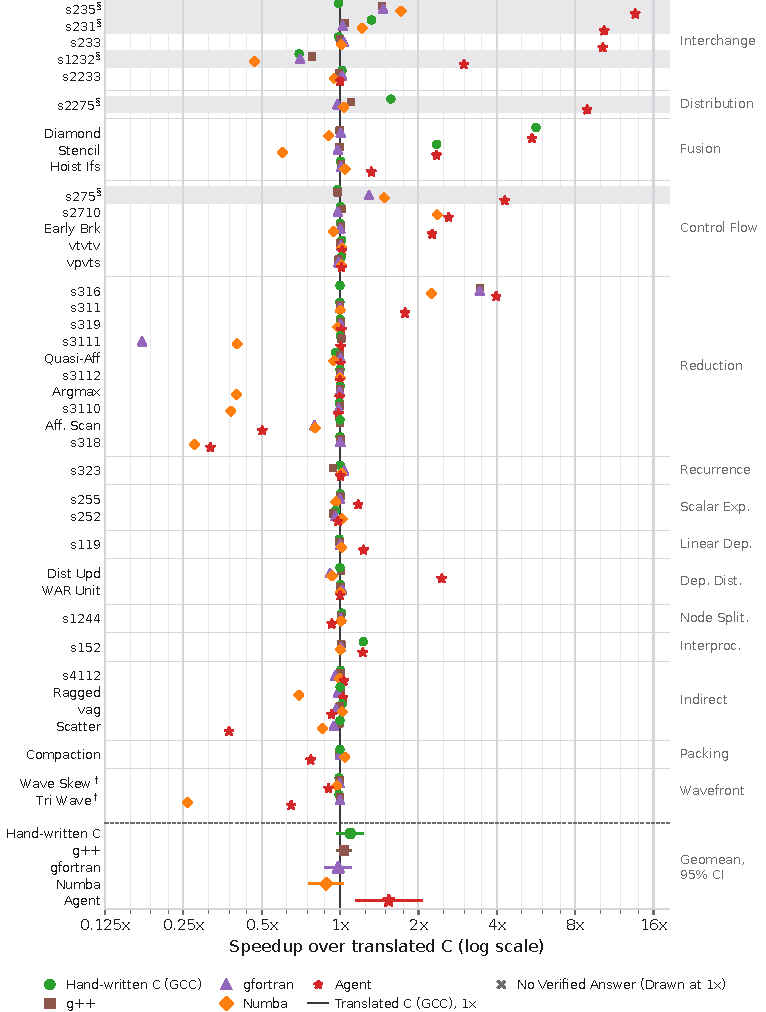
\includegraphics[width=\textwidth]{figures/llr40_speedup.pdf}
  \caption{Speedup of each version over the translated C version of the same kernel, at preset M
    on one core of a GH200 node (minimum of 30 runs). Kernels are grouped by transformation class;
    the bottom rows give each column's geometric mean with its 95\% interval. A hollow cross at
    1$\times$ marks a missing version. \texttt{s115} is not shown, because no GCC version
    produces a valid result at this size. $^\dagger$The two wavefront kernels pass validation
    only vacuously at preset M, as explained at the end of this section. $^\S$Shaded rows: the
    GCC versions did not reproduce between two measurements (\Cref{sec:setup}), so differences
    between them are memory-bandwidth noise.}
  \label{fig:llr40-speedup}
\end{figure}

\begin{table}[t]
  \centering
  \small
  % Generated by plotting/thesis/llr40_matrix.py -- do not edit.
\begin{tabular}{@{}lrcrrr@{}}
  \toprule
  Column & $n$ & Speedup over C (95\% CI) & Faster & Tie & Slower \\
  \midrule
  Hand-written C (GCC) & 34 & 1.10$\times$ [0.97, 1.24] & 5 & 26 & 3 \\
  g++ & 39 & 1.04$\times$ [0.97, 1.11] & 4 & 32 & 3 \\
  gfortran & 39 & 0.98$\times$ [0.87, 1.11] & 5 & 26 & 8 \\
  Numba & 39 & 0.88$\times$ [0.76, 1.03] & 8 & 15 & 16 \\
  Agent & 38 & 1.54$\times$ [1.14, 2.07] & 18 & 12 & 8 \\
  \bottomrule
\end{tabular}

  \caption{Geometric-mean speedup of each column over translated C, over the kernels where both
    are valid, with the number of kernels on which the column is more than 3\% faster, within
    3\%, or more than 3\% slower.}
  \label{tab:llr40-geomean}
\end{table}

\paragraph{The language matters little on a shared backend.}
Translated into C, C++ and Fortran and compiled by GCC, the same kernel runs at nearly the same
speed. Neither g++ (1.04$\times$ the speed of translated C) nor gfortran (0.98$\times$) differs
from C beyond its 95\% interval, and the three agree within 5\% on 27 of 39 kernels; five of the
other twelve are the unstable kernels of \Cref{sec:setup}. GCC's optimisation reports show why:
its vectorisation decisions for the three translated languages differ on only four of the 39
kernels, and only one of these differences changes the run time. No language wins
consistently: among the four translated versions, Numba is fastest on 13 kernels, C++ on 12,
Fortran on 8 and C on 6.

\paragraph{The large gaps are individual code-generation decisions.}
Where the languages do differ, each gap traces to one decision in the generated code, not to the
language. On \texttt{s3111}, a conditional sum, gfortran is 5.8$\times$ slower than C. The
translator writes every accumulation in parentheses, \texttt{sum = (sum + a(i))}, and in Fortran
parentheses are binding, so gfortran keeps them and does not recognise the reduction. Removing
only the parentheses makes it vectorise the loop. The same parentheses prevent an FMA in the
recurrence of \texttt{scan\_affine\_decay}, where Fortran is 1.25$\times$ slower. On
\texttt{s316}, a running minimum, it is C that is 3.4$\times$ slower than C++ and Fortran,
although the C and C++ sources are identical. GCC 14, which compiles the C columns, turns the
update into a branch-free select that puts the comparison on the loop-carried dependence chain,
while GCC 13 keeps a branch that almost never mispredicts on random data. Rebuilding the same
sources with the other compiler version swaps the behaviour, so the difference is the compiler
version, not the language. The protocol had expected the opposite effect on reductions: that
gfortran's licence to reassociate would make Fortran faster. In the matrix, gfortran vectorises
none of the ten reductions.

\paragraph{Numba's results are LLVM's.}
Numba is the most uneven column: faster than C on 8 kernels, slower on 16, and 0.88$\times$ the
speed of C overall. It is 2.4$\times$ faster than C on \texttt{s2710}, a loop with nested branches that LLVM
vectorises using SVE predication. GCC gives up on a single statement: a test of \texttt{x[0]}, a
scalar that the translator passes as a one-element array and reads inside the loop. Because it
is read in only one branch, GCC neither hoists it out of the loop nor vectorises the masked load
it becomes. It
is 2.5 to 3.6$\times$ slower on the four reductions whose update is conditional
(\texttt{s318}, \texttt{s3110}, \texttt{argmax\_with\_index}, \texttt{s3111}): LLVM turns the
conditional update into the same branch-free select that slows the C version of \texttt{s316},
while GCC keeps a branch or, on \texttt{s3111}, vectorises. Whether a compiler
implements a loop-carried comparison as a branch or as a select is the single most frequent
cause of a large gap in the matrix, and it decides kernels in both directions.

\paragraph{A value carried through memory costs about six cycles.}
The second recurring mechanism is whether a value carried from one iteration to the next stays
in a register or is stored and immediately loaded again. In \texttt{versioned\_distance\_update},
graded at distance $K = 1$, the translated C version stores \texttt{a[i]} and loads it back as
\texttt{a[i-K]} in the next iteration. Because $K$ is known only at run time, GCC cannot keep the
value in a register, and the check with which it versions the loop for vectorisation always fails
at $K = 1$. The loop runs at 10.4 cycles per element. The agent version tests for $K = 1$ and
keeps the value in a register, which leaves only the latency of the FMA on the critical path:
4.2 cycles per element, 2.5$\times$ faster. \texttt{wf\_triangular} shows the same effect
between GCC and Numba. GCC keeps the neighbour \texttt{a[i, j-1]} in a register and runs at 2.1
cycles per element, the latency of one addition. Numba stores and reloads it, because its address
passes through the wraparound that Python semantics require for a negative index, and runs at
8.2 cycles. In both kernels the round trip through memory adds about six cycles per element, which is
consistent with the latency of forwarding a store to the next load on this core.

\paragraph{No compiler restructures; the agents do.}
In the five interchange kernels and the distribution kernel, GCC's optimisation reports contain
no interchange and no distribution in any column. Where they are strided, GCC considers the
inner loops for vectorisation and rejects them on cost. For \texttt{s231}, where the interchange is
legal, GCC's interchange pass did not even take up the loop nest as a candidate. The agents
interchanged, distributed or flattened these loops by hand, after which GCC vectorised the
unit-stride inner loop they had produced; this makes the agent version 3.0 to 9.9$\times$
faster than the fastest other version. Four of these kernels are among the unstable ones, but
the agent versions are not: they access memory with unit stride and vary by at most 2\% from run
to run. The hand-written C column shows the same effect from
the other side. It ties translated C on 26 of 34 kernels, but is 5.6$\times$ faster on
\texttt{fuse\_diamond} and 2.3$\times$ faster on \texttt{fuse\_stencil\_through\_transient}. There
the hand-written reference is the original, already fused TSVC loop, while the NumPy reference,
and hence every translated version, is deliberately unfused, and GCC does not fuse it. On these
kernels the hand-written column is the optimised answer, not a baseline.

\paragraph{Agent code carries its target machine.}
The agent column is the fastest overall (1.54$\times$ the speed of C), but slower than C on
eight kernels. In the submissions we inspected, the cause is parallel scaffolding that costs
work when it runs on one thread. The
submission for \texttt{scan\_affine\_decay} is a three-pass blocked parallel scan that reads its
input twice, and is 2.0$\times$ slower than the sequential recurrence. The one for
\texttt{scatter\_accum\_dup} hard-codes the MI300A node it was written on: 48 threads, 24 cores
per rank, pinning to SMT siblings, and atomic compare-and-swap updates. It overrides the
single-thread setting and is 2.7$\times$ slower. Portability fails more directly elsewhere: for
12 of the 13 kernels where we could not use the campaign's best submission, that submission
included x86 intrinsics headers and does not compile on an Arm machine. A speedup an agent
achieved on its own machine does not by itself transfer to another one.

\paragraph{Vectorising is not the same as being fast.}
According to its optimisation reports, GCC vectorises a loop in 15 of 39 kernels in the C
column, 12 in the Fortran column and 27 in the agent column; Numba's assembly contains vector
loops for 19 kernels. On this machine a vector instruction holds only two \texttt{float64}
values: GCC mostly uses 128-bit Advanced SIMD vectors and SVE in only a few loops, mostly where it
needs predication, and Grace implements SVE with 128-bit vectors too. Vectorisation alone can
therefore gain at most about 2$\times$, while the restructuring in the agent versions changes how
the loops traverse memory. Vectorising alone does not predict speed either. On the plain sum \texttt{s311}, GCC vectorises the C version as an
in-order SVE reduction, yet it runs exactly as fast as the scalar Fortran version (135\,ms),
because an in-order reduction is still bound by the latency of its additions. Only the agent's
OpenMP reduction, which permits reassociation, is faster (76\,ms). This agrees with what Bonsall
and Budanaz~\cite{bonsall2026dace} observed for code generated by DaCe.

\paragraph{Floating-point contraction decides correctness.}
\label{par:fma}
\texttt{s115} accumulates values that span hundreds of orders of magnitude, so at preset M its
output is almost entirely infinite or NaN. With \texttt{-ffp-contract=fast}, GCC fuses its
multiply-subtract into an FMA, which rounds differently from NumPy's separate operations and
changes where the overflow occurs, so all four GCC versions fail validation. With
\texttt{-ffp-contract=off}, and nothing else changed, all four pass. Numba passes in both cases
because it never enables \texttt{fastmath} and reproduces NumPy's arithmetic exactly. The two
wavefront kernels overflow as well, but consist only of additions, so every version produces
the same mostly non-finite output and passes vacuously. At the largest sizes whose output is
fully finite (118 for \texttt{s115}, 517 and 1017 for the wavefronts), every version passes, and
the wavefront timings show the same pattern as at preset M: Numba 3.6$\times$ and the agent
1.6$\times$ slower than C on \texttt{wf\_triangular}.

% TODO: the extracted kernels, measured under the same protocol at the same benchmark commit.
% Integer kernels are graded bit-exact, so the floating-point effects above apply only to WarpX
% and QuaTrEx; the hand-written column is upstream C++ for CoMet, WarpX and NFA, unsupported for
% the CUDA references (SpGEMM, triangle counting).

\section{Skill Evaluation}
% Kernel extraction: extract a kernel with and without the skill; score fidelity
% (validation layers passed, boundary choice, documented simplifications).
% Preconditioning: three scenarios (frozen preconditioner, binding cap, disagreement) on
% the solver test kernels, with and without the skill; baseline failures without it.
% TODO: run both.

\section{Discussion}
% Representation, compiler or algorithm: on LLR-40 the language explains little; the spread
% comes from code-generation decisions (backend, compiler version, translator emission) and from
% restructuring, which only the agents supplied. Revisit with the extracted kernels.
% Branch versus select on a loop-carried comparison as the recurring decision; register versus
% memory for a loop-carried value (about 6 cycles of store-to-load forwarding) as the second.
% Translator recommendations: hoist loop-invariant scalars passed as one-element arrays (s2710);
% do not emit binding parentheses around Fortran accumulations (s3111, scan_affine_decay).
% Hypothesis to check on daint: GCC refuses every conditional min/max reduction ("unsupported use
% in stmt") because it may only form MIN/MAX_EXPR when NaNs can be ignored (-ffinite-math-only),
% which the oracle forbids -- i.e. the grading itself removes this optimisation.
% What elementwise grading permits: FP contraction as a correctness choice; reassociation only
% via an explicit reduction clause; vacuous passes on numerically degenerate kernels.
% Threats to validity: single thread and one machine; GCC is the only C/C++/Fortran compiler
% (LLVM only through Numba); C built by GCC 14, C++ and Fortran by GCC 13; agent column produced
% on MI300A and run serially; small classes and disputed labels; -ftree-parallelize-loops
% checked and without effect (geomean 1.00, no loop parallelised).
